% \documentclass[a4paper,twoside,twocolumn,10pt]{article}
\documentclass[a4paper,twoside,twocolumn,10pt]{jarticle}     %pLaTeX2e仕様(platex.exeの場合)
\usepackage{abstract} % Style for abstracts in Dept. CSIS, OPU
%\usepackage{abstract4past} % Style for abstracts for the past curriculum

%%%%%%%%%% Designate packages you need %%%%%%%%%%
% \usepackage{graphicx} % Enhanced support for graphics
\usepackage[dvipdfm]{graphicx}
\usepackage{url} % Verbatim with URL-sensitive line breaks
\usepackage{multirow}
%%%%%%%%%% Parameters that should be customized %%%%%%%%%%
% Language (1 = Japanese, 2 = English)
\setlang{1}
% Bachelor or Master (1 = Bachelor, 2 = Master)
\setborm{1}
% Fiscal year
\setfy{2020}
% Group number
\setgnum{1}
% Presentation order
\setorder{4}
% Increase page number (optional)
%% \pplus{1}

% Title
\title{深層学習に基づく 4 コマ漫画の感情推定と\\マルチモーダル化への検討}
% Author
\author{高山 裕成}
%%%%%%%%%% Parameters that should be customized (end) %%%%%%%%%%

\begin{document}
\maketitle % Insert title
\small

\section{はじめに}
近年, 深層学習を始めとする機械学習技術の大きな発展を受けて, 人工知能を用いた創作物理解が注目されている.
しかし, 創作は高次の知的活動であるため, いまだに実現が困難なタスクである.
人の創作物理解に関する分野の中でも漫画を対象とした研究は,
絵と文章から構成される漫画を対象とする自然言語処理と画像処理の両方の側面を持つマルチモーダルデータを扱う分野である.
漫画を対象とした研究分野では様々な研究が報告されているが,
その多くは画像処理に基づいた研究であり,
自然言語処理による内容理解を目指した研究は少ない.

本研究では, 人工知能を用いた漫画の内容理解のために,
まず自然言語処理を用いて漫画のキャラクタのセリフの感情を推定する.
その上で漫画のコマの画像情報を加えたマルチモーダルな推定手法について検討する.
そして, 実験結果からセリフの感情推定とマルチモーダル化の精度への影響について考察した.
%%%%%%%%%%%%%%%%%%%%%%%%%%%%%%
\section{要素技術}
\subsection{BERT}
Bidirectional Encoder Representations from Transformers (BERT)
 \cite{devlin2018bert} は, 2018 年に Google が発表した言語モデルであり,
 文書分類や質疑応答といった様々な自然言語処理の幅広いタスクにおいて公開時点での最高性能を達成している. 本研究では日本語 Wikipedia によって事前学習させたモデル \cite{kyoto-bert} (以下, 京大 BERT) 及び, 大規模日本語 SNS コーパスによって事前学習させたモデル, hottoSNS-BERT \cite{hottoSNS-bert} を用いた.

\subsection{illustration2vec}
illustration2vec \cite{i2v} は Saito, Matsui らが提案した画像のベクトル化手法である. 既存の画像認識モデルのほとんどが実画像を評価対象にしているのに対し, Saito らの手法はアニメや漫画といったイラストに対して評価しており, 漫画やイラストのより合理的なベクトル化が期待できる. 本研究では筆者らが公開している事前学習済みモデルを用いた.
%%%%%%%%%%%%%%%%%%%%%%%%%%%%%%
\section{提案手法}
本研究では, 上野によって作られた 4 コマ漫画ストーリーデータセット \cite{ueno_miki2018} を用いて,
各セリフにアノテートされた感情ラベルを推定するタスクを解き, その精度を確認する.

図 \ref{fig:teian} にマルチモーダルな推定手法として, 提案手法の概要を示す.
Text Embedding 層への入力として, あるセリフを選んだ時に, Image Embedding 層への入力をこのセリフが含まれているコマの画像全体とする. そして, それぞれの層から得たものをセリフベクトルとコマベクトルとし, これらを結合したものを識別器への入力とすることでセリフの感情ラベルを推定する.

\begin{figure}[!th]
  \centering
  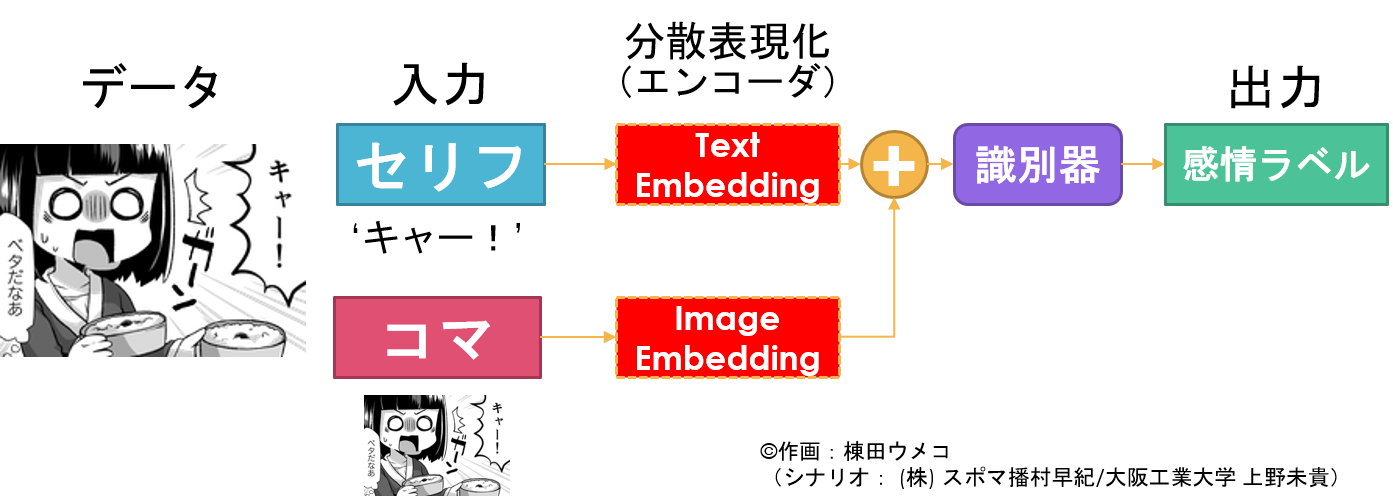
\includegraphics[scale=0.25]{teian.png}
  \caption{提案手法の概要}
  \label{fig:teian}
\end{figure}
%%%%%%%%%%%%%%%%%%%%%%%%%%%%%%
\section{実験}
本研究で用いるデータセットには 7 種類の感情ラベルと,
アノテーション不備によって感情ラベルが不明なデータが含まれているが,
データ数と解析の難しさの問題から感情ラベルが不明なデータを除き, ``喜楽" のみを正例, その他の感情ラベルを負例とする 2 クラスに分類し, これを推定した. ベースラインとしては, 偏ったラベル比の問題からすべての出力が負例と推定された場合の評価指標の値を設定した. また Image Embedding 層から得たコマベクトルは固定し, Text Embedding 層には前述した 2 種類の BERT モデルを用いて精度を比較した. 識別器としては 3 層 MLP を用いた. 実験 1 ではセリフ 1 文のみを入力とし, 対応する感情ラベルを推定した. 実験 2 では提案手法に則って, マルチモーダルな感情推定の検討をした.

表 \ref{table:result} に各実験の精度 (Acc), および正例の F 値 (P-F 値) を示す. 各実験において, どちらの BERT モデルを用いても Acc はベースラインを超え, 評価指標は hottoSNS-BERT の方が上回った. 実験 2 の結果から, どちらの BERT モデルを用いても P-F 値は上がっており, コマベクトルを加えることで, 文字だけでは人間の目で見ても判断が難しいものが一部識別できるようになった.

% 実験 1 ではセリフ 1 文のみを入力とし, 対応する感情ラベルを推定した. 実験の結果, どちらの BERT モデルを用いても全体の精度はベースライン (70.5\%) を超えた. (京大 BERT : 73.3\%, hottoSNS-BERT : 75.8\%) また, hottoSNS-BERT の方が, より正例を識別できていた.
%
% 実験 2 では提案手法に則って, マルチモーダルな感情推定の検討をした. 実験の結果, hottoSNS-BERT では全体の精度は実験 1 を上回った. (京大 BERT : 71.5\%, hottoSNS-BERT : 77.6\%) また, どちらの BERT モデルを用いても正例の識別率は上がった. コマベクトルを加えることで, 文字だけでは人間の目で見ても判断が難しいものが一部識別できるようになった.

\begin{table}[h]
\vspace{-2mm}
\begin{center}
\caption{実験結果}
\scalebox{0.6}{
\begin{tabular}{llcc}
                                           &               & Acc                       & P-F 値 \\ \hline
\multicolumn{1}{l|}{\multirow{2}{*}{実験 1}} & 京大 BERT       & 0.733                     & 0.535 \\
\multicolumn{1}{l|}{}                      & hottoSNS-BERT & 0.758                     & 0.586 \\ \hline
\multicolumn{1}{l|}{\multirow{2}{*}{実験 2}} & 京大 BERT       & 0.715                     & 0.546 \\
\multicolumn{1}{l|}{}                      & hottoSNS-BERT & 0.776                     & 0.622 \\ \hline
                                           & ベースライン        & \multicolumn{1}{l}{0.705} & -
\end{tabular}
\label{table:result}
}
\end{center}
\vspace{-10mm}
\end{table}

%%%%%%%%%%%%%%%%%%%%%%%%%%%%%%
\section{まとめと今後の課題}
本研究ではマルチモーダルな感情推定が漫画に対しても有効であることを確認した. また, hottoSNS-BERT を用いることでセリフのより合理的な分散表現が得られた. 今後の課題として, セリフベクトルとコマベクトルの結合方法の最適化などが挙げられる. そして, 他のデータセットを併用した半教師あり学習や人手によるデータセット拡張についても検討していく必要がある.


\bibliographystyle{jabbrvunsrt}
\bibliography{index_ja}
\end{document}
